\documentclass[12pt]{article}
\usepackage{amsmath}
\usepackage{bm}
\usepackage{siunitx}
\usepackage{parskip}
\usepackage{graphicx}
\usepackage[letterpaper, margin=1in]{geometry}
\usepackage{fancyhdr}
\usepackage{gensymb}
\fancypagestyle{prelabheader} {
    \rhead{Raeed Hassan \\ hassam41}
    \lhead{\huge{ELECENG 2CI5 Lab 8 Prelab}}
}
\graphicspath{{./images/}}

\begin{document}
\newgeometry{margin=1in, includehead, head=47pt}
\thispagestyle{prelabheader}
i.
For a series circuit such as this, the current through all the components of the circuit is this same. This means we can simply find the current through inductor by solving the current through the circuit. This current can be found by getting the phaser of the current, which is the phaser of the voltage divided by the total impedance in the circuit.
\[
    \tilde{I} = \frac{\tilde{V}}{z} \\
\]
The total impedance in the circuit is the sum of the impedance through the resistor and the impedance through the inductor.
\[
\begin{gathered}
    z = z_{R_1} + z_{L_1} \\
    z = R_1 + j\omega L_1 \\
    z = R_1 + j\cdot2\pi\cdot f\cdot L_1\\
    z  = 100 + j\cdot 2\pi \cdot 1\times10^5 \cdot 1\times10^{-3} \\
    z = 100 + j200\pi \\
\end{gathered}
\]
To find the the current phaser, we need to determine the modulus and angle of the impedance and divide the voltage by the impedance 
\[
\begin{gathered}
    \left|z\right| = \sqrt{100^2 + 200^2} = 636.2\\
    \angle \theta_z = \arctan(\frac{200\pi}{100}) = 1.41\; rad \\
    \tilde{I} = \frac{\tilde{V}}{z} = \frac{V_m\angle \theta_v}{\left|z\right| \angle \theta_z} = \frac{V_m}{\left|z\right|} \angle \theta_v - \theta_z \\
    \tilde{I} = \frac{1}{636.2} \angle 0\;rad - 1.41\;rad = 1.57mA\; \angle -1.41\; rad \\
\end{gathered}
\]
The phaser of the current can simply be converted to the sinusodial equation representating the current with respect to time.
\[
    I_L(t) = 1.57\cos(20000\pi t - 1.41)\; mA
\]
\restoregeometry
\clearpage
ii.
\begin{center}
    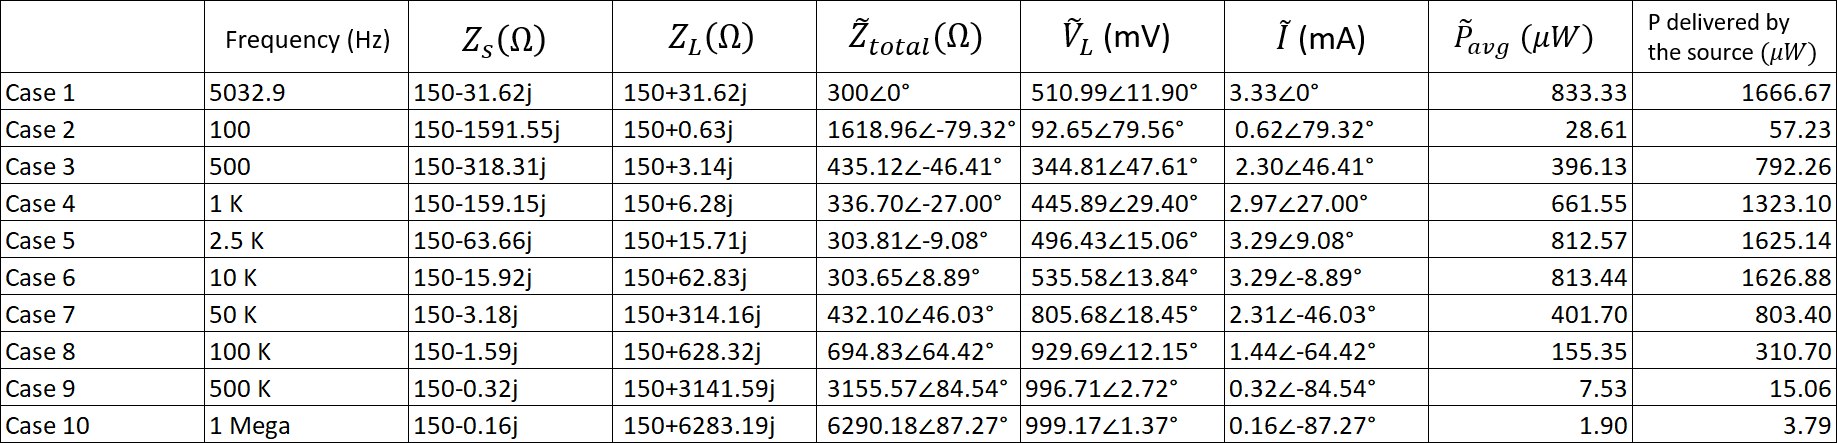
\includegraphics[width=\textwidth]{q2.PNG}
\end{center}

iii. \\
The amplitude of the inductor current is approximately 1.57mA.

iv. 
\begin{center}
    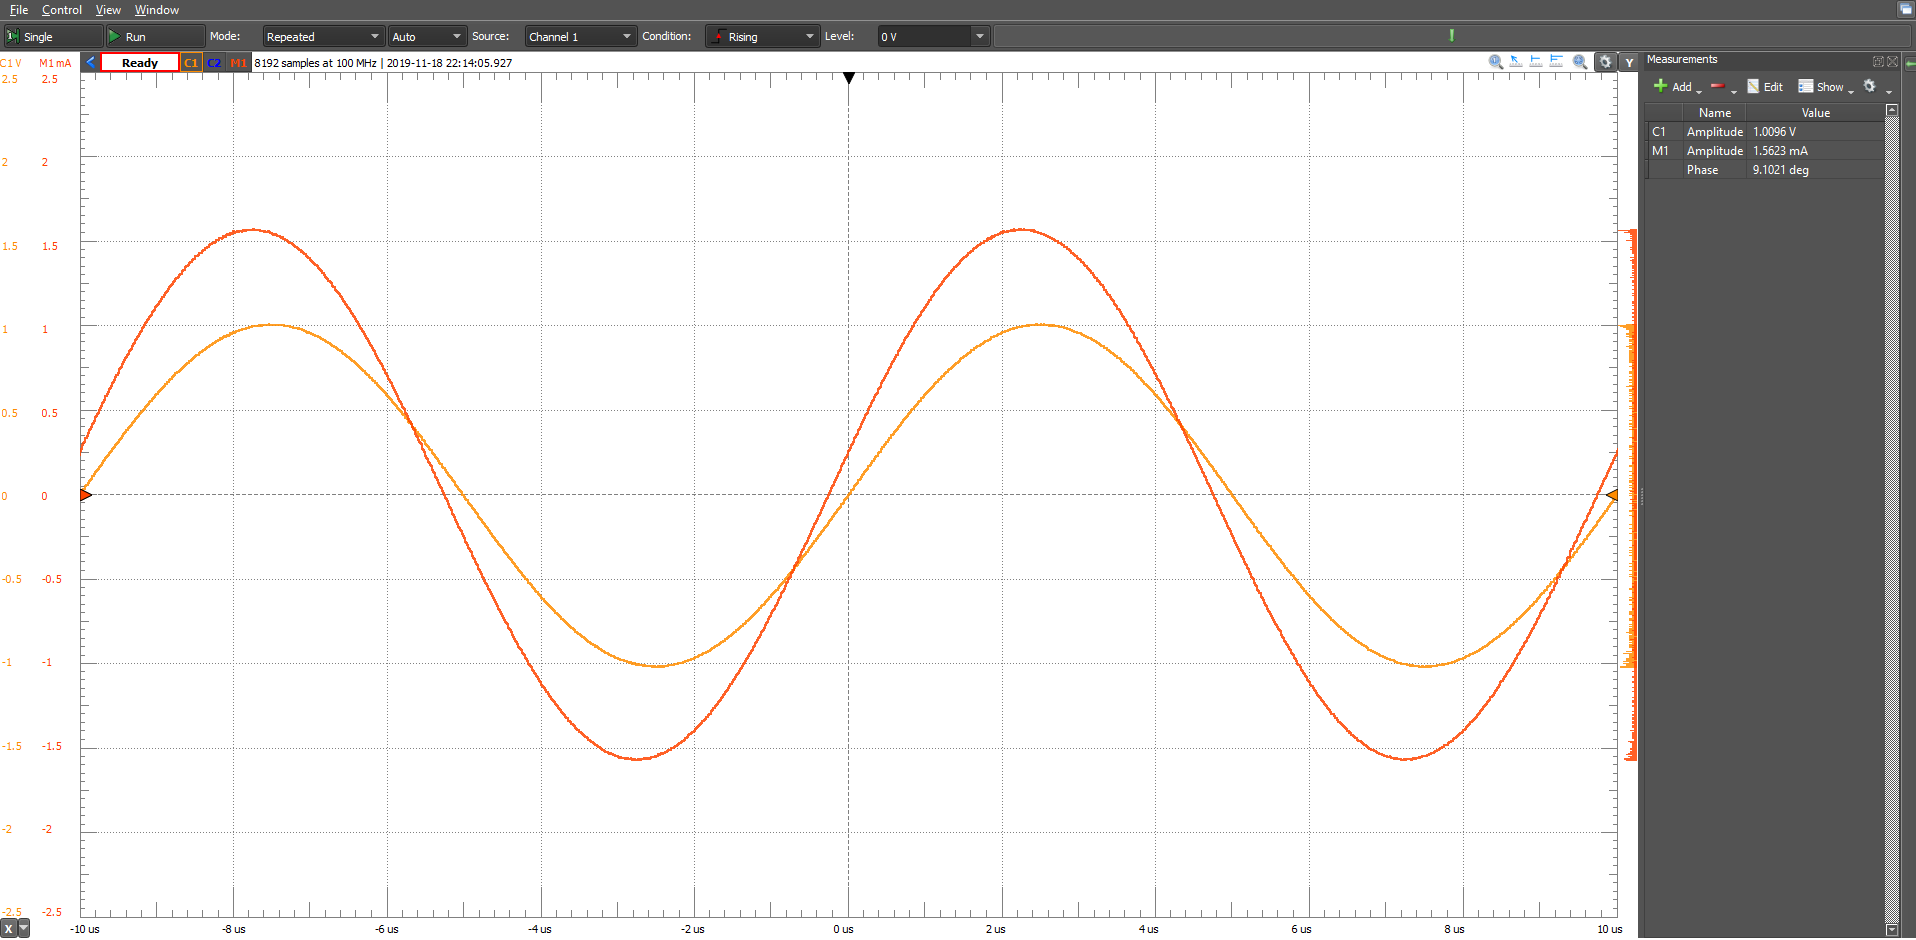
\includegraphics[width=\textwidth]{q4.png}
\end{center}
v. \\
The phase difference is $-81$\degree or -1.41 rad.

vi. \\
The three waveforms shared the same amplitude and angular frequency. The only difference between the some waveforms were their phase. The calculated waveform and the actual waveform both had a phase difference of $-1.41$ rad, while the simulated waveform had a phase difference of $-\dfrac{\pi}{2}$ rad or -1.57 rad.

vii.\\
When the input is set to resonance frequency in a series RLC circuit, the imaginary component of the impedance is zero, as the imaginary components of the impedance caused the inductor and capacitor cancel each other out. This represents the lowest possible impedance for the circuit, the highest possible current for the circuit, and the highest possible voltage for the resistor.
\end{document}